\chapterhead{6}{What the Diagram Leaves Out}{Asking what a picture of the cycle can and cannot tell us}\label{ch6}

A diagram of the water cycle is a model. It keeps the order of the stages and drops almost everything else: the places, the times, the amounts, the plants, the ice. Whether a model is good depends on the question you ask of it.

\begin{center}
\sffamily\small\renewcommand{\arraystretch}{1.5}
\begin{tabular}{@{}p{3.4cm}p{3.7cm}p{3.7cm}@{}}
\toprule
\textbf{Model} & \textbf{What it keeps} & \textbf{What it drops}\\
\midrule
A level in a cup & how much water is there & where the missing water went\\
A ledger & the total across places & the path between them\\
A colour test & whether drops came from inside & tiny leaks that carry no colour\\
A solar still & the order of the changes & real sea, real sky, real time\\
A cycle diagram & the order of the stages & times, places, amounts\\
\bottomrule
\end{tabular}
\end{center}

\subhead{A question for every model}
Ask of any diagram: what question is it for? Then ask: what would it get wrong if I used it for a different question?

\begin{tryit}{A rain gauge}
\textbf{You need:} a straight-sided clear cup or jar, a ruler marked in mm, a spot outdoors away from trees.
\begin{enumerate}[leftmargin=1.6em]
\item Stand the cup outside before rain is due, level on the ground or a flat shelf.
\item Each day at the same time, measure the depth of water in mm. Then empty the cup.
\item Write the readings for a week.
\end{enumerate}
\par\medskip
\renewcommand{\arraystretch}{1.6}
\begin{tabular}{|l|c|c|c|c|c|c|c|}
\hline
\textbf{Day} & Mon & Tue & Wed & Thu & Fri & Sat & Sun\\ \hline
\textbf{Rain (mm)} & & & & & & & \\ \hline
\end{tabular}
\end{tryit}

\begin{worked}{Practice numbers, not from a real week}
Mon 4, Tue 0, Wed 7, Thu 2, Fri 0: total $4+0+7+2+0=13$~mm in five days.\\
The average is $13\div5=2.6$, about 3~mm a day.\\
Each 1~mm of rain is 1 litre of water on every square metre of ground. So 13~mm is 13 litres on each square metre.
\end{worked}

\begin{multix}[hmm]\multixbot[hmm]\tcblower
The diagram has five boxes and five arrows, so it must be a perfect picture of the real sky. I trust it for everything. Am I being careful?
\end{multix}

\trust{We asked what question the diagram is meant to answer, then checked it against real measurements, a jar, a bowl and a rain gauge.}
{The diagram gets the order of the stages right, and the small tests kept their totals.}
{Anything about how long water stays, how much falls in a place, or how much goes where. For those questions we need other models, such as a ledger with numbers.}

\begin{keepbox}
We turned a week of rain into one number. \textbf{We kept} \wline[3.4cm] \textbf{and we set aside} \wline[3.4cm].
\end{keepbox}

\clearpage

\begin{puzzle}{Rain total}
Rain gauge readings: 5, 0, 3, 6, 1~mm. Total \wline[1.6cm]~mm \quad Average per day \wline[1.6cm]~mm
\end{puzzle}

\begin{puzzle}{Which question?}
Mark Y if the five-box diagram can answer the question and N if it cannot.\\
(a) What stage comes after the cloud? \wline[1cm]\\
(b) How long does a drop stay in the air? \wline[1cm]\\
(c) How much rain falls on my town? \wline[1cm]
\end{puzzle}

\begin{puzzle}{Improve the diagram}
Name one thing you would add to the diagram to make it answer a new question, and the question. \wline[6cm]
\end{puzzle}

\begin{puzzle}{Weather clue}
Match each clue to a stage. E (evaporation), C (condensation) or R (rain falling).\\
(a) Washing dries on a line \wline[1cm] \quad (b) A cold can gets wet outside \wline[1cm]\\
(c) A puddle appears under grey clouds \wline[1cm]
\end{puzzle}

\begin{puzzle}{Wrap the claim}
A student writes ``the water in the open cup vanished''. Use what you know to wrap that claim with a better one. \wline[6cm]
\end{puzzle}

\clearpage

\begin{puzzle}{Ledger check}
A cup started with 30 spoonfuls and ended with 22. How many moved into the air? \wline[1.6cm]
\end{puzzle}

\begin{puzzle}{Unfair rain test}
Ben put one rain gauge under a tree and another in an open field. They read 2~mm and 9~mm. He says the field gets more rain. What is wrong with the test? \wline[6cm]
\end{puzzle}

\begin{puzzle}{Model or real thing?}
Write M for model and R for real thing.\\
(a) A drawing of the cycle \wline[1cm] \quad (b) A cloud \wline[1cm] \quad (c) A closed jar with a plant \wline[1cm]
\end{puzzle}

\begin{puzzle}{One question}
Write a question that a ledger can answer but a five-box diagram cannot. \wline[6cm]
\end{puzzle}

\clearpage

\begin{puzzle}{Rain again}
8, 0, 0, 4, 3~mm. Total \wline[1.6cm]~mm
\end{puzzle}

\begin{puzzle}{Missing step}
Water went from the sea to a cloud. Name the step in between. \wline[3cm]
\end{puzzle}

\begin{puzzle}{A cold morning}
The outside of a cold bottle gets wet in a warm kitchen. Name the change. \wline[3cm]
\end{puzzle}

\begin{puzzle}{Trust}
A student says her jar kept all its water, so water is never lost anywhere. What should she check? \wline[6cm]
\end{puzzle}

\clearpage

\begin{puzzle}{Draw the move: the lake}
A lake loses 6 units to the air on a sunny day. Draw a move from the lake to the air and write the amount. Then write what the lake and the air hold now if they held 100 and 20 at the start.
\begin{center}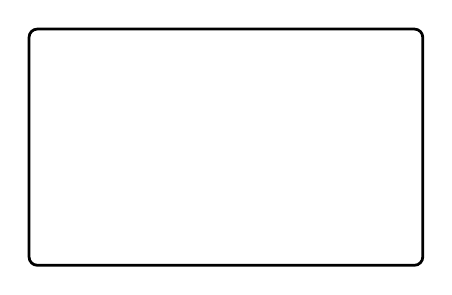
\begin{tikzpicture}\draw[line width=1pt,rounded corners=3pt] (0,0) rectangle (5,3); \end{tikzpicture}\end{center}
\end{puzzle}

\begin{puzzle}{Draw the loop: the bag}
Draw the cloud-in-a-bag loop with circles: water, vapour, drops. Label the steps.
\begin{center}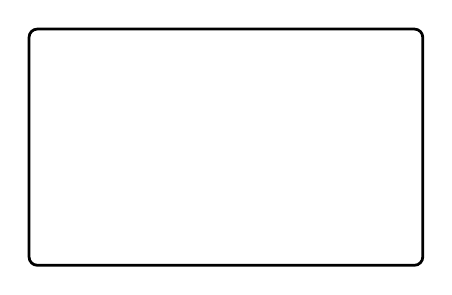
\begin{tikzpicture}\draw[line width=1pt,rounded corners=3pt] (0,0) rectangle (5,3); \end{tikzpicture}\end{center}
\end{puzzle}

\begin{puzzle}{Draw the wrap}
Draw a circle around ``water vanished'' and write the corrected claim outside it.
\begin{center}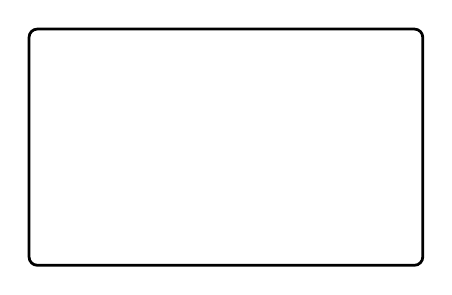
\begin{tikzpicture}\draw[line width=1pt,rounded corners=3pt] (0,0) rectangle (5,3); \end{tikzpicture}\end{center}
\end{puzzle}

\clearpage
\thispagestyle{fancy}\label{slop}
\subhead{Slop check}
Slop is hasty, gaudy work that forgot to take care. It can be made by a person or a machine, quickly or slowly. What matters is whether the work shows care for three things:
\begin{itemize}[leftmargin=1.6em]
\item \textbf{Salient:} Is the main point easy to see?
\item \textbf{Simple:} Is there anything that does nothing but get in the way?
\item \textbf{Relevant:} Does everything on the page help answer the question?
\end{itemize}

Here is a hasty poster about rain. Study it, then decide what is wrong.

\begin{center}
\begin{tikzpicture}[scale=0.97]
  \fill[yellow!40,draw=purple!80!black,line width=3pt] (0,0) rectangle (11.4,7.6);
  \node[star,star points=12,fill=red!60,draw=blue,line width=2pt,minimum size=2.2cm,font=\bfseries\scriptsize,rotate=10,text=yellow] at (1.4,6.2) {WOW!!!};
  \node[font=\itshape\bfseries\Large,text=teal,rotate=-4] at (6.4,6.8) {RaIn Is MaGiC};
  \node[font=\ttfamily\tiny,text=orange] at (6.4,6.15) {(water maybe? who knows)};
  \foreach \x/\h/\c in {3/1.2/red,5.3/3.2/blue,7.6/5.0/green}{
    \fill[\c,draw=black] (\x,0.9) rectangle (\x+1.3,0.9+\h);
  }
  \node[font=\tiny,text=black,rotate=60] at (9.8,3) {number number number};
  \foreach \x/\y in {1.2/1.5,1.6/4.2,10.2/5.6,0.8/3}{\node[star,star points=5,fill=yellow,draw=red,minimum size=0.6cm] at (\x,\y) {};}
  \node[font=\tiny,text=lime!50!black] at (5.4,0.45) {look at it!!!  best rain ever!!!  wow  wow};
\end{tikzpicture}
\end{center}

\begin{slopbox}
\textbf{(a)} What is the poster's main point? Can you tell?\\[3pt]\rule{\linewidth}{0.5pt}\\[6pt]
\textbf{(b)} Name two things that are not simple, because they only distract.\\[3pt]\rule{\linewidth}{0.5pt}\\[6pt]
\textbf{(c)} Name two things that are missing, so the bars cannot be read.\\[3pt]\rule{\linewidth}{0.5pt}\\[6pt]
\textbf{(d)} Which part is not relevant to rain at all?\\[3pt]\rule{\linewidth}{0.5pt}
\end{slopbox}

\clearpage
\thispagestyle{fancy}
\subhead{Now you try}
On a separate sheet, redraw a clear bar chart of rain each day: Mon 4~mm, Tue 0~mm, Wed 7~mm, Thu 2~mm, Fri 0~mm. Give it a title, label the axes with units, use one or two calm colours, and delete everything that does not help. Check it against the three words: salient, simple, relevant.

\begin{center}
\begin{tikzpicture}
  \draw[ink!70,line width=1pt,rounded corners=3pt] (0,0) rectangle (11.4,1.0);
  \node[font=\sffamily\small,anchor=west] at (0.2,0.5) {Title:};
  \draw[line width=1.3pt] (1,1.6) -- (1,9.6);\draw[line width=1.3pt] (1,1.6) -- (11,1.6);
  \foreach \y in {2.6,3.6,...,8.6}{\draw[gray!40] (1,\y) -- (11,\y);}
  \node[font=\sffamily\scriptsize,rotate=90] at (0.3,5.6) {label and unit here};
  \node[font=\sffamily\scriptsize] at (6,1.3) {label what the axis stands for};
\end{tikzpicture}
\end{center}

\clearpage
\thispagestyle{fancy}
\subhead{What did we keep, across the whole book?}
For each chapter, say one thing that was simplified, what was kept, and what was set aside. A sample is done for you.

\renewcommand{\arraystretch}{2.3}
\begin{center}\sffamily\scriptsize
\begin{tabularx}{\textwidth}{|>{\bfseries}p{2.1cm}|X|X|X|}
\hline
\textbf{Chapter} & \textbf{What we simplified} & \textbf{What we kept} & \textbf{What we set aside} \\ \hline
1 Level in a cup & the water as a height in mm & how much is left & where it went \\ \hline
2 Drying up & drying as minutes & which dries sooner & the path of the vapour \\ \hline
3 Cold glass & drops as one number & whether they were clear & the size of each drop \\ \hline
4 A cup with a lid & water as spoonfuls & the total & the exact path \\ \hline
5 The long loop & the cycle as boxes & the order & times and amounts \\ \hline
6 The diagram & & & \\ \hline
\end{tabularx}
\end{center}

\begin{multix}[wow]\multixbot[wow]\tcblower
Everything you drew in this book was a simplification of something. A model is allowed to drop things, as long as you say which. Next time a puddle shrinks, you will know where it went.
\end{multix}

\clearpage
\thispagestyle{fancy}
\subhead{Write a water report}
\begin{tcolorbox}[enhanced,colback=white,colframe=ink!60,boxrule=1pt,arc=2mm,left=8pt,right=8pt,top=5pt,bottom=5pt]
\sffamily\small
\begin{enumerate}[leftmargin=1.6em,itemsep=0.2em]
\item \textbf{What I looked at.}
\item \textbf{What I changed, measured and kept the same.}
\item \textbf{My readings.} All of them.
\item \textbf{My answer.} With averages and spread.
\item \textbf{What I kept and what it hides.}
\end{enumerate}
\end{tcolorbox}
\vspace{4pt}
Pick one test from this book and write a report on it. Use the lines below.\par\medskip
\foreach \i in {1,...,12}{\rule{\linewidth}{0.4pt}\\[18pt]}
\clearpage

\thispagestyle{fancy}
\subhead{Tests to try}
Pick one and design it with the habits from this book: change one thing, keep the rest the same, repeat, and average.
\begin{enumerate}[leftmargin=1.6em,itemsep=0.5em]
\item Does the wind make a wet towel dry faster? Try a fan or a breezy window.
\item Does the shape of a dish change how fast water evaporates?
\item Does salty water evaporate faster or slower than fresh water?
\item How long does it take a cold can to form drops in different rooms?
\item Does a plant in a closed jar keep the jar's water for longer than an open one?
\item How much rain falls on different spots around your home?
\end{enumerate}
\medskip
Write the test you pick:\par\medskip
\foreach \i in {1,...,6}{\rule{\linewidth}{0.4pt}\\[16pt]}
Change: \wline[3cm] Measure: \wline[3cm] Keep the same: \wline[3cm]
\clearpage

\thispagestyle{fancy}
\subhead{A week of water}
Each day, notice one place water goes in or out of the air and say which stage it is.\par\medskip
\renewcommand{\arraystretch}{3.2}
\begin{tabularx}{\linewidth}{|>{\sffamily\small\bfseries}p{1.8cm}|X|X|}
\hline
Day & What I saw & Which stage \\ \hline
Mon & & \\ \hline
Tue & & \\ \hline
Wed & & \\ \hline
Thu & & \\ \hline
Fri & & \\ \hline
Sat & & \\ \hline
Sun & & \\ \hline
\end{tabularx}
\clearpage

\thispagestyle{fancy}
\subhead{Questions I still have}
Write what you still wonder about water. Then pick one and think how to test it.\par\medskip
\foreach \i in {1,...,16}{\rule{\linewidth}{0.4pt}\\[16pt]}
\clearpage
